\documentclass[11pt,a4paper]{article}
\usepackage{fontspec}
\setmainfont{TeX Gyre Pagella}
\newfontfamily\headfont{Inter}[UprightFont=*-ExtraBold,BoldFont=*-ExtraBold,Extension=.otf,Path=/usr/share/fonts/opentype/inter/]
\usepackage[a4paper,margin=2.3cm]{geometry}
\usepackage{graphicx,booktabs,float,caption,array,xcolor,longtable}
\usepackage{xurl}
\usepackage[hidelinks]{hyperref}
\usepackage{titlesec}
\usepackage[round]{natbib}
\usepackage{setspace}
\setstretch{1.05}
\renewcommand{\topfraction}{0.9}
\renewcommand{\bottomfraction}{0.8}
\renewcommand{\textfraction}{0.1}
\renewcommand{\floatpagefraction}{0.75}
\setlength{\parindent}{0pt}
\setlength{\parskip}{0.55em}
\titleformat{\section}{\headfont\Large}{\thesection}{0.8em}{}
\titleformat{\subsection}{\headfont\large}{\thesubsection}{0.8em}{}
\captionsetup{font=small,labelfont=bf}
\urlstyle{same}
\hypersetup{pdftitle={Fencing the Commons},pdfauthor={Tristan Hotham}}

\begin{document}
\begin{center}
{\Large\bfseries Fencing the Commons\par}
\vspace{0.4em}
{\large Mapping parliamentary enclosure in England and Wales\\from the Chronological Tables of Private and Local Acts\par}
\vspace{1.2em}
{\large Tristan Hotham\par}
\vspace{0.3em}
{\small Independent researcher\\
ORCID: 0000-0003-4931-9349\\
DOI: https://doi.org/10.5281/zenodo.23873003\par}
\vspace{0.8em}
2026
\end{center}

\begin{quote}
\small
\begin{center}\textbf{Abstract}\end{center}
I extract every enclosure Act listed in the Chronological Tables of Private and Personal Acts and of Local Acts published on legislation.gov.uk, place the parishes and townships they name on the map, and describe when and where parliamentary enclosure happened in England and Wales. The tables list 3,655 private Acts and 449 local Acts that enclosed open fields, commons or wastes, from 1562 to 1873. I geocode 4,259 of the 5,375 places they name (79\%) against a Wikidata gazetteer, locating 3,431 Acts. The Acts come in two waves: 985 private Acts in the 1760s and 1770s, peaking at 87 in 1777, and 1,967 Acts in the 23 years of war with France from 1793 to 1815, peaking at 125 in 1811. The war years account for 48\% of all the Acts. From 1799 a growing share of enclosure Acts appears in the local table rather than the private one (about half in 1811 to 1814), so the second wave is visible only when both tables are combined. Enclosure by Act was concentrated in a Midland belt: twelve counties with 21\% of England's area had 39\% of its private enclosure Acts, led by Northamptonshire with 7.5 Acts per 100 km$^2$, while Kent, Devon and Cornwall, long enclosed by other means, had 15, 26 and 1. The second wave was not a repeat of the first: the Midland belt's share of Acts fell from 53\% to 31\%, while Norfolk and Suffolk, the south-west and the Welsh border, the home counties and Wales all gained. The centre of gravity of enclosure moved about 46 km, from near Nottingham in the 1760s to west of Leicester in the 1810s.

\textbf{Keywords:} enclosure; inclosure Acts; open fields; common rights; agrarian history; England; Wales; French wars; historical GIS; legislation.gov.uk
\end{quote}

\section{Introduction}
Parliamentary enclosure turned much of what remained of England's open fields, commons and wastes into privately held, hedged fields between the middle of the eighteenth century and the middle of the nineteenth. Where the owners of a parish could not or would not enclose by agreement, a private Act of Parliament appointed commissioners who surveyed the parish, extinguished common rights, and allotted the land in severalty. The history of the process has been written county by county, above all in W. E. Tate's list of Acts and awards \citep{tate1978} and Michael Turner's historical geography \citep{turner1980}, and its effects have been argued over for more than a century, from the Hammonds' account of the labourer's losses \citep{hammond1911} to Chambers and Mingay's account of agricultural progress \citep{chambers1966}, Allen's reassessment of the gains \citep{allen1992} and Neeson's study of common right \citep{neeson1993}.

This paper does something narrower and more mechanical. It takes the Chronological Tables of Private and of Local Acts as published by legislation.gov.uk \citep{legpriv,legloc}, extracts every enclosure Act, places the parishes and townships named in each title on the map using open data \citep{wikidata}, and describes the resulting pattern in time and space. Everything is reproducible from the published tables, and an interactive map accompanies the paper (\url{https://maps.tristanhotham.com/enclosure/}).

\section{Data}
\textbf{The private table.} The Chronological Table of Private and Personal Acts lists every private Act from 1539 to 1987 by session and chapter, with a short title, in 33 parts. I use all 33 parts (12,284 rows). A typical enclosure entry reads ``c. 1 Turvey (Bedfordshire) inclosure.'', under a session heading such as ``1783 (23 Geo. 3).''.

\textbf{The local table.} The Chronological Table of Local Acts begins in 1797. Its enclosure titles rarely give a county (``c.vii Upton and Fishley Inclosures.''). I use 185 of its 187 pages; the parts for 1802 to 1803 and for 1841 could not be collected, and only headings and rows mentioning inclosure were kept (483 rows).

\textbf{The gazetteer.} About 49,500 rows from Wikidata describe places in the United Kingdom with a coordinate, a type (civil parish, village, town, hamlet) and, for most, a historic county. After merging repeated rows and keeping England and Wales, 28,035 places remain. Cornish places, which lack a historic county in Wikidata, are assigned to Cornwall by the modern county outline; a few others take the county of their nearest neighbours.

\section{Methods}
\subsection{Reading the tables}
Titles that run over two rows are rejoined, and annotation rows recording later repeals, amendments and savings (``r.-'', ``am.-'', ``see:'', ``saved in pt.-'') are dropped with their run-on lines. Each Act is dated by the first calendar year of its session heading. Every title containing a word beginning ``inclos'' or ``enclos'' is kept: 3,722 private and 483 local titles. Each is classed as an enclosure Act (the usual ``Place (County) inclosure'', including drainage and inclosure, inclosure with tithe exchange or commutation, and commons inclosure), an Act confirming an inclosure already agreed (51 private Acts, counted with the enclosure Acts), an amendment (43 private Acts that only explain, amend or extend an earlier Act), a confirmation of the Inclosure Commissioners' provisional orders (29 local Acts after 1845), or other titles that mention enclosing in passing. Ten Acts for Irish counties are excluded. The result is 3,655 private and 449 local enclosure Acts. A further 68 private titles speak only of allotment or division and are not counted.

\subsection{Places and geocoding}
The text before a title's first county is split into places on commas and ``and'', keeping compound names (``Great and Little Cressingham'' becomes Great Cressingham and Little Cressingham) and alternative spellings (``North Hykeham or Hickham''). Each place is matched to the gazetteer within the county or counties the title names, using a normalised key (Saint and St., upon and on, juxta and next, possessives and hyphens). When there is no exact match, the parish is tried for a piece of land named within it (``Glusburn Moor in Kildwick''), the first township of a compound name, and a unique longer name (Goring for Goring-on-Thames). Old spellings are matched by string similarity (ratio at least 0.88) only when one candidate is clearly best. Ambiguous names are settled only by another place in the same Act within 20 km. A unique name in a neighbouring county within 15 km is accepted, which recovers parishes in detached parts of counties such as Norham and Blockley. Places in local Acts without a county are matched only when the name is unique in England and Wales or settled by a neighbour. Table~\ref{tab:geo} summarises the matches; every unmatched place is listed with the data.

\begin{table}[tbp]\centering\small\caption{How the named places of enclosure Acts were matched to the gazetteer.}\label{tab:geo}\begin{tabular}{lrr}\toprule Match & Places & Share\\\midrule
Exact name in the county & 3,475 & 64.7\%\\
Parish or main name of a compound & 234 & 4.4\%\\
Close spelling in the county & 442 & 8.2\%\\
Ambiguous, settled by a neighbour & 90 & 1.7\%\\
Unique name just over a county boundary & 18 & 0.3\%\\
Ambiguous, left unmatched & 210 & 3.9\%\\
Not found & 906 & 16.9\%\\
\midrule All named places & 5,375 & 100\%\\
\bottomrule\end{tabular}\end{table}

\subsection{Counties and areas}
An Act is counted for the first county its title names, or, if it names none, for the county of its first located place. There is no historic county boundary file among the inputs, so I rebuild one: a Voronoi cell around every gazetteer place, merged by historic county and clipped to the coast. The resulting areas match the historic counties closely (Yorkshire 15,648 km$^2$, Rutland 379 km$^2$) and are used for densities. Yorkshire is treated as one county.

\subsection{Periods, regions and centroids}
The French wars are taken as 1793 to 1815 inclusive. The first wave is compared over 1750 to 1779. Regions are groups of historic counties: the Midland belt (Northamptonshire, Leicestershire, Oxfordshire, Cambridgeshire, Huntingdonshire, Bedfordshire, Buckinghamshire, Warwickshire, Rutland, Nottinghamshire, Lincolnshire and Berkshire), the north (Northumberland, Cumberland, Westmorland, Durham, Yorkshire and Lancashire), the south-west and Welsh border (Cornwall, Devon, Somerset, Dorset, Wiltshire, Hampshire, Gloucestershire, Herefordshire, Shropshire and Worcestershire), Norfolk and Suffolk, the home counties and Kent (Kent, Sussex, Surrey, Middlesex, Essex and Hertfordshire), and Wales. The centroid of a decade is the mean British National Grid position of its located Acts, each Act placed at the mean of its located places.

\section{Results}
\subsection{Two waves}
Figure~\ref{fig:years} shows the Acts per year. Before 1750 there are 113 enclosure Acts. The first wave brought 147 private Acts in the 1750s, 359 in the 1760s and 626 in the 1770s, with a peak of 87 in 1777. The 1780s were quieter (229 Acts, with 11 in 1784). The war years brought 1,967 Acts, 85.5 a year against 49.2 a year in 1760 to 1779. Private Acts peaked at 100 in 1801; with local Acts included, every year from 1809 to 1814 saw more than 100, and 1811 saw 125. The 1800s were the busiest decade (850 Acts), followed by the 1810s (803). The end of the war ended the boom: 114 Acts in 1814, 79 in 1815 and 43 in 1816. Of the private Acts, 43\% came before 1793, 42\% in the war years and 15\% after; of the local Acts, 95\% came in the war years (Figure~\ref{fig:eras}).

\begin{figure}[tbp]\centering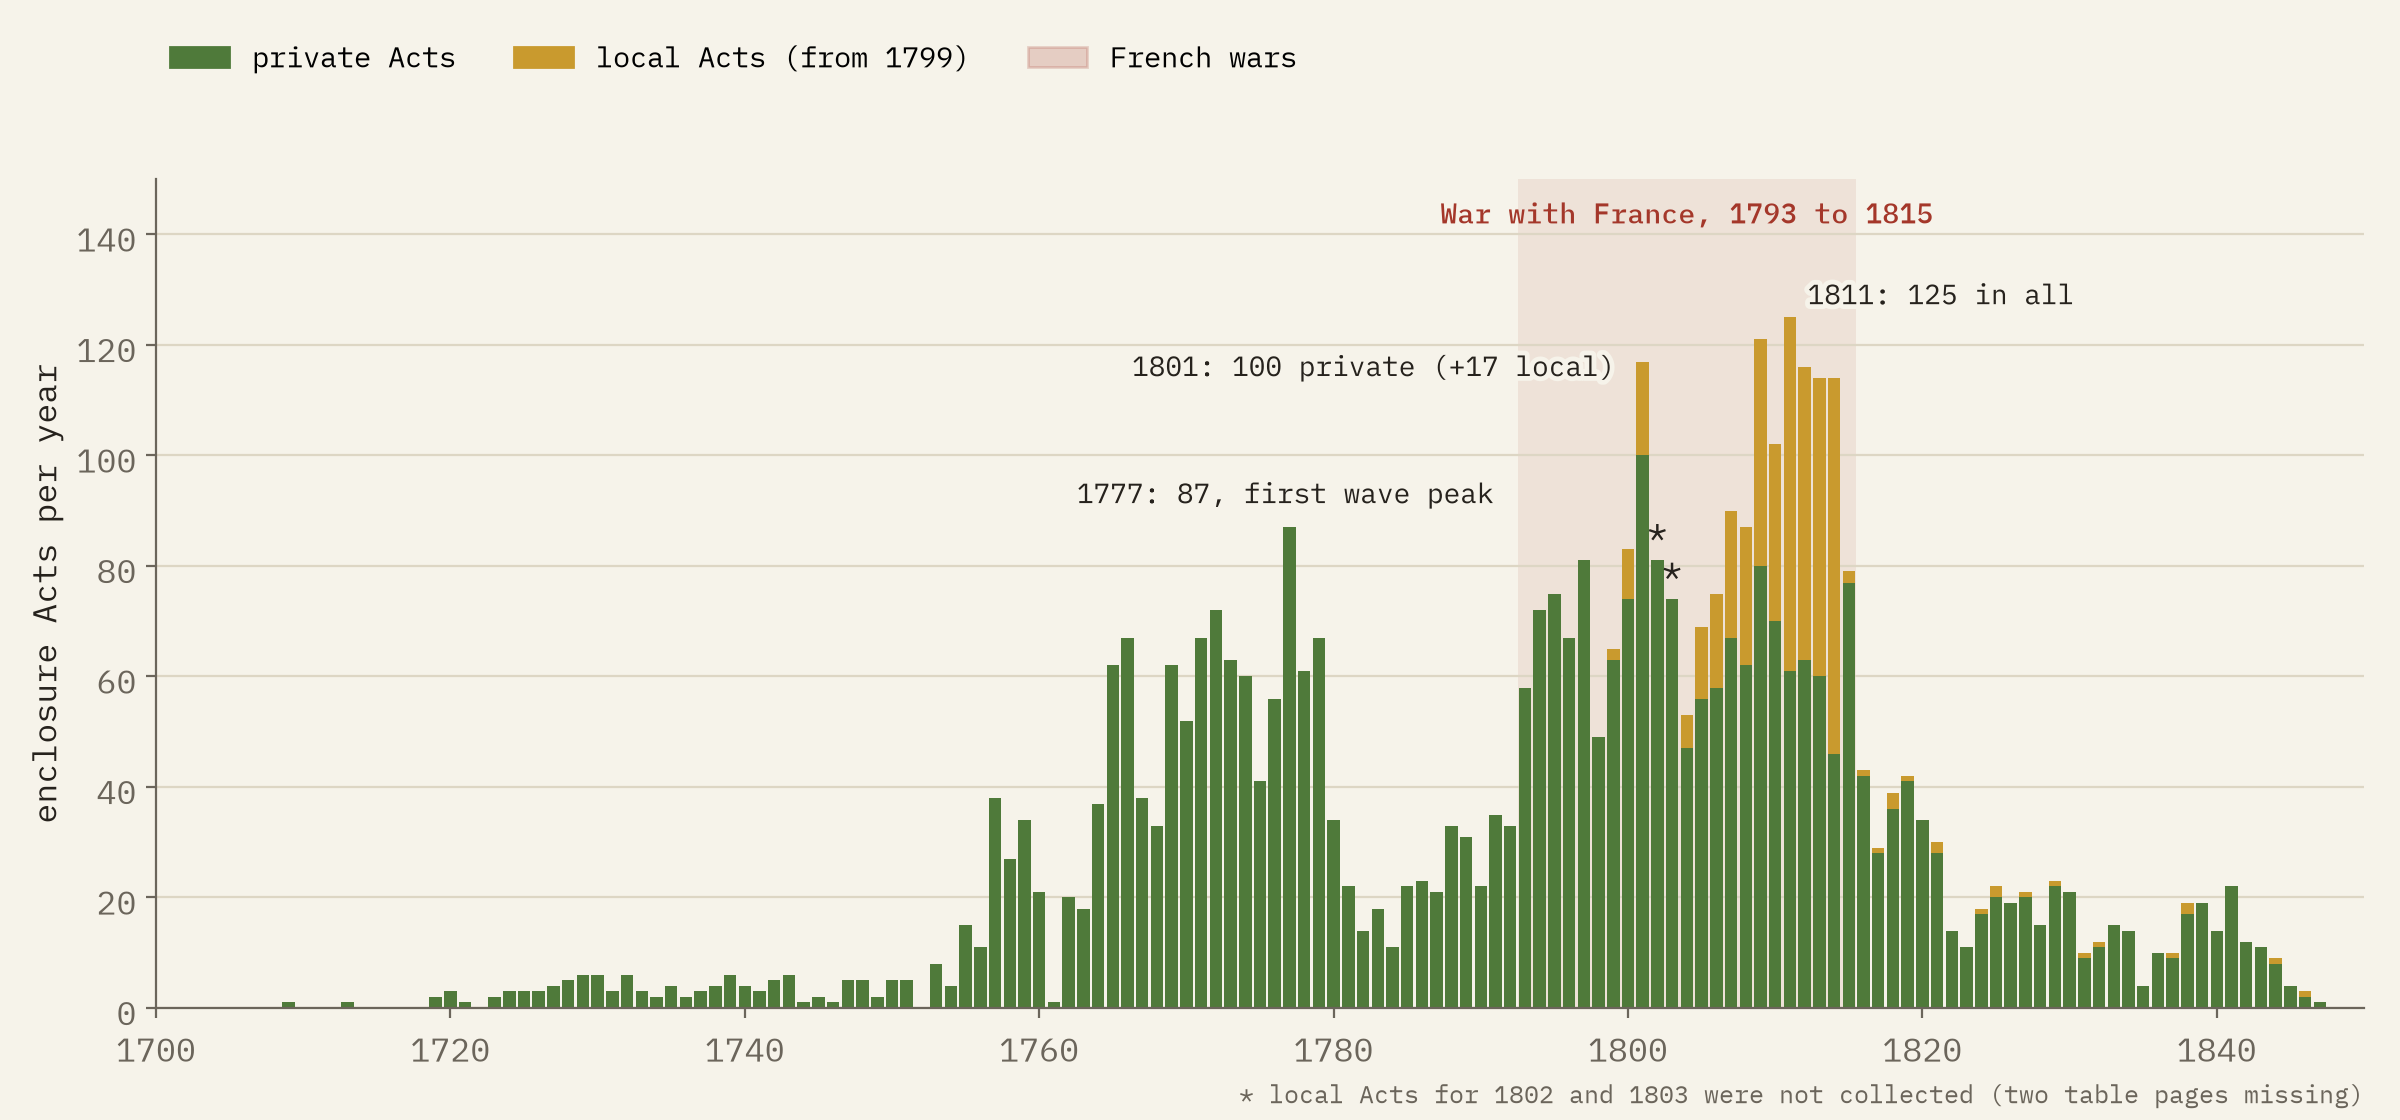
\includegraphics[width=\textwidth]{f_years.png}
\caption{Enclosure Acts per year, 1700 to 1849: private Acts (green) and local Acts (gold), with the French wars shaded. Local Acts for 1802 and 1803 were not collected.}\label{fig:years}\end{figure}

\begin{figure}[tbp]\centering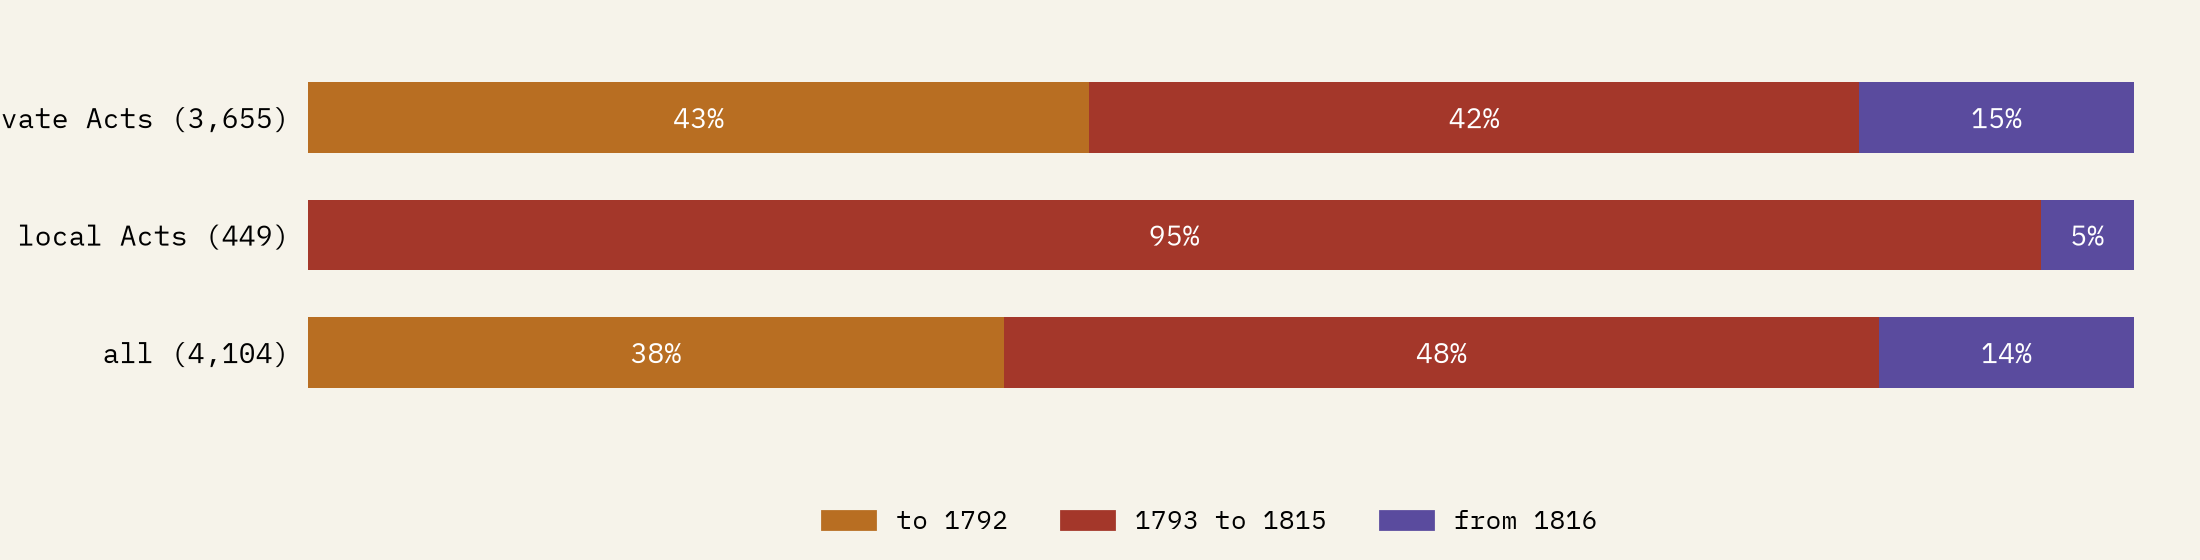
\includegraphics[width=\textwidth]{f_eras.png}
\caption{Share of enclosure Acts before, during and after the French wars.}\label{fig:eras}\end{figure}

The split between the tables matters. Local enclosure Acts appear from 1799; 426 of them were passed by 1815, 26\% of all enclosure Acts in 1798 to 1815 and 51\% in 1811 to 1814. Counting private Acts alone would show the second wave peaking in 1801 and declining thereafter, which is an artefact of classification.

\subsection{Where}
Figure~\ref{fig:map} maps the 4,259 located places and Figure~\ref{fig:counties} the density of private Acts by county; Table~\ref{tab:counties} gives the figures. Northamptonshire (7.50 Acts per 100 km$^2$), Leicestershire (6.93), Rutland (6.60), Huntingdonshire (6.00) and Nottinghamshire (5.82) lead. The Midland belt has 1,399 private Acts on 27,014 km$^2$, 5.18 per 100 km$^2$ against 2.73 for England. At the other end, Kent (0.37), Devon (0.38) and Cornwall (0.03) rank 44th, 43rd and last of 52 counties, as expected for counties enclosed early by agreement or with little open field. Essex and Sussex are also low. By number rather than density, Yorkshire has the most Acts (544 private), then Lincolnshire (265) and Norfolk (219). Wales has 70 private and 92 Acts in all, 60\% of its private Acts in the war years. The Midland counties were enclosed earliest: the middle year of Leicestershire's Acts is 1772, of Northamptonshire's 1778, against 1807 for Norfolk and 1813 for Devon.

\begin{figure}[tbp]\centering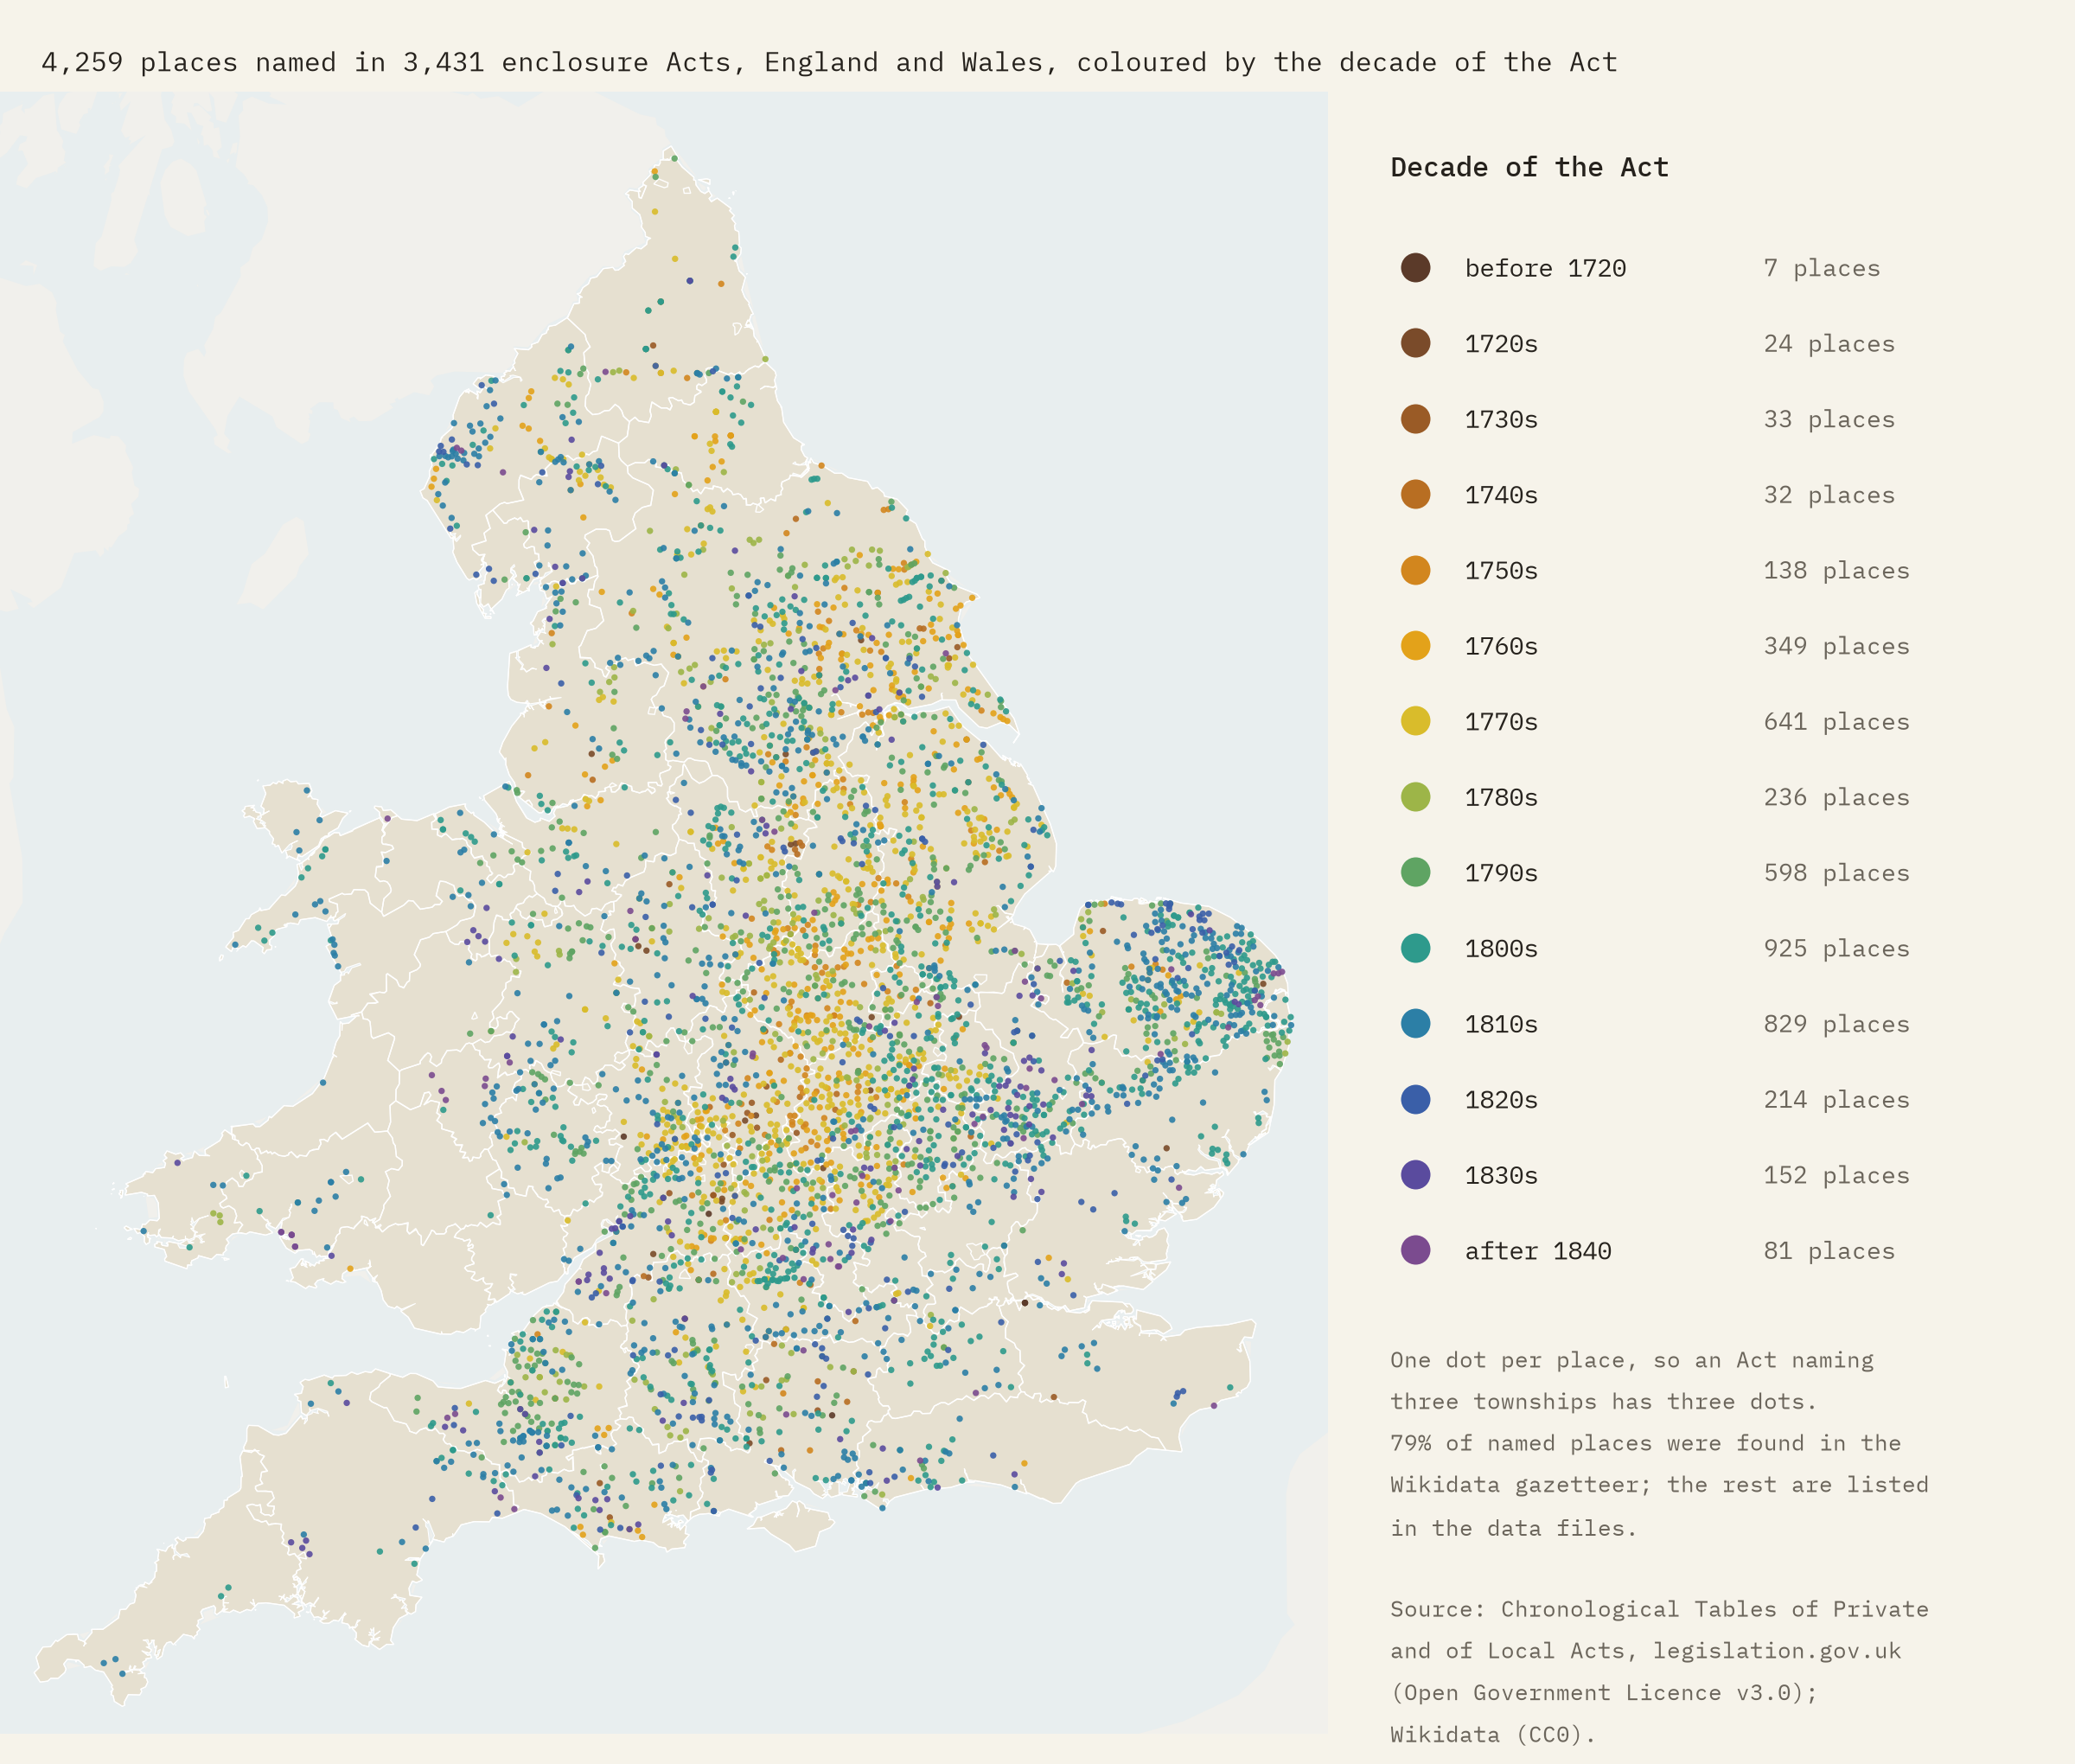
\includegraphics[width=\textwidth]{f_map.png}
\caption{Places named in enclosure Acts and found in the gazetteer, coloured by the decade of the Act.}\label{fig:map}\end{figure}

\begin{figure}[tbp]\centering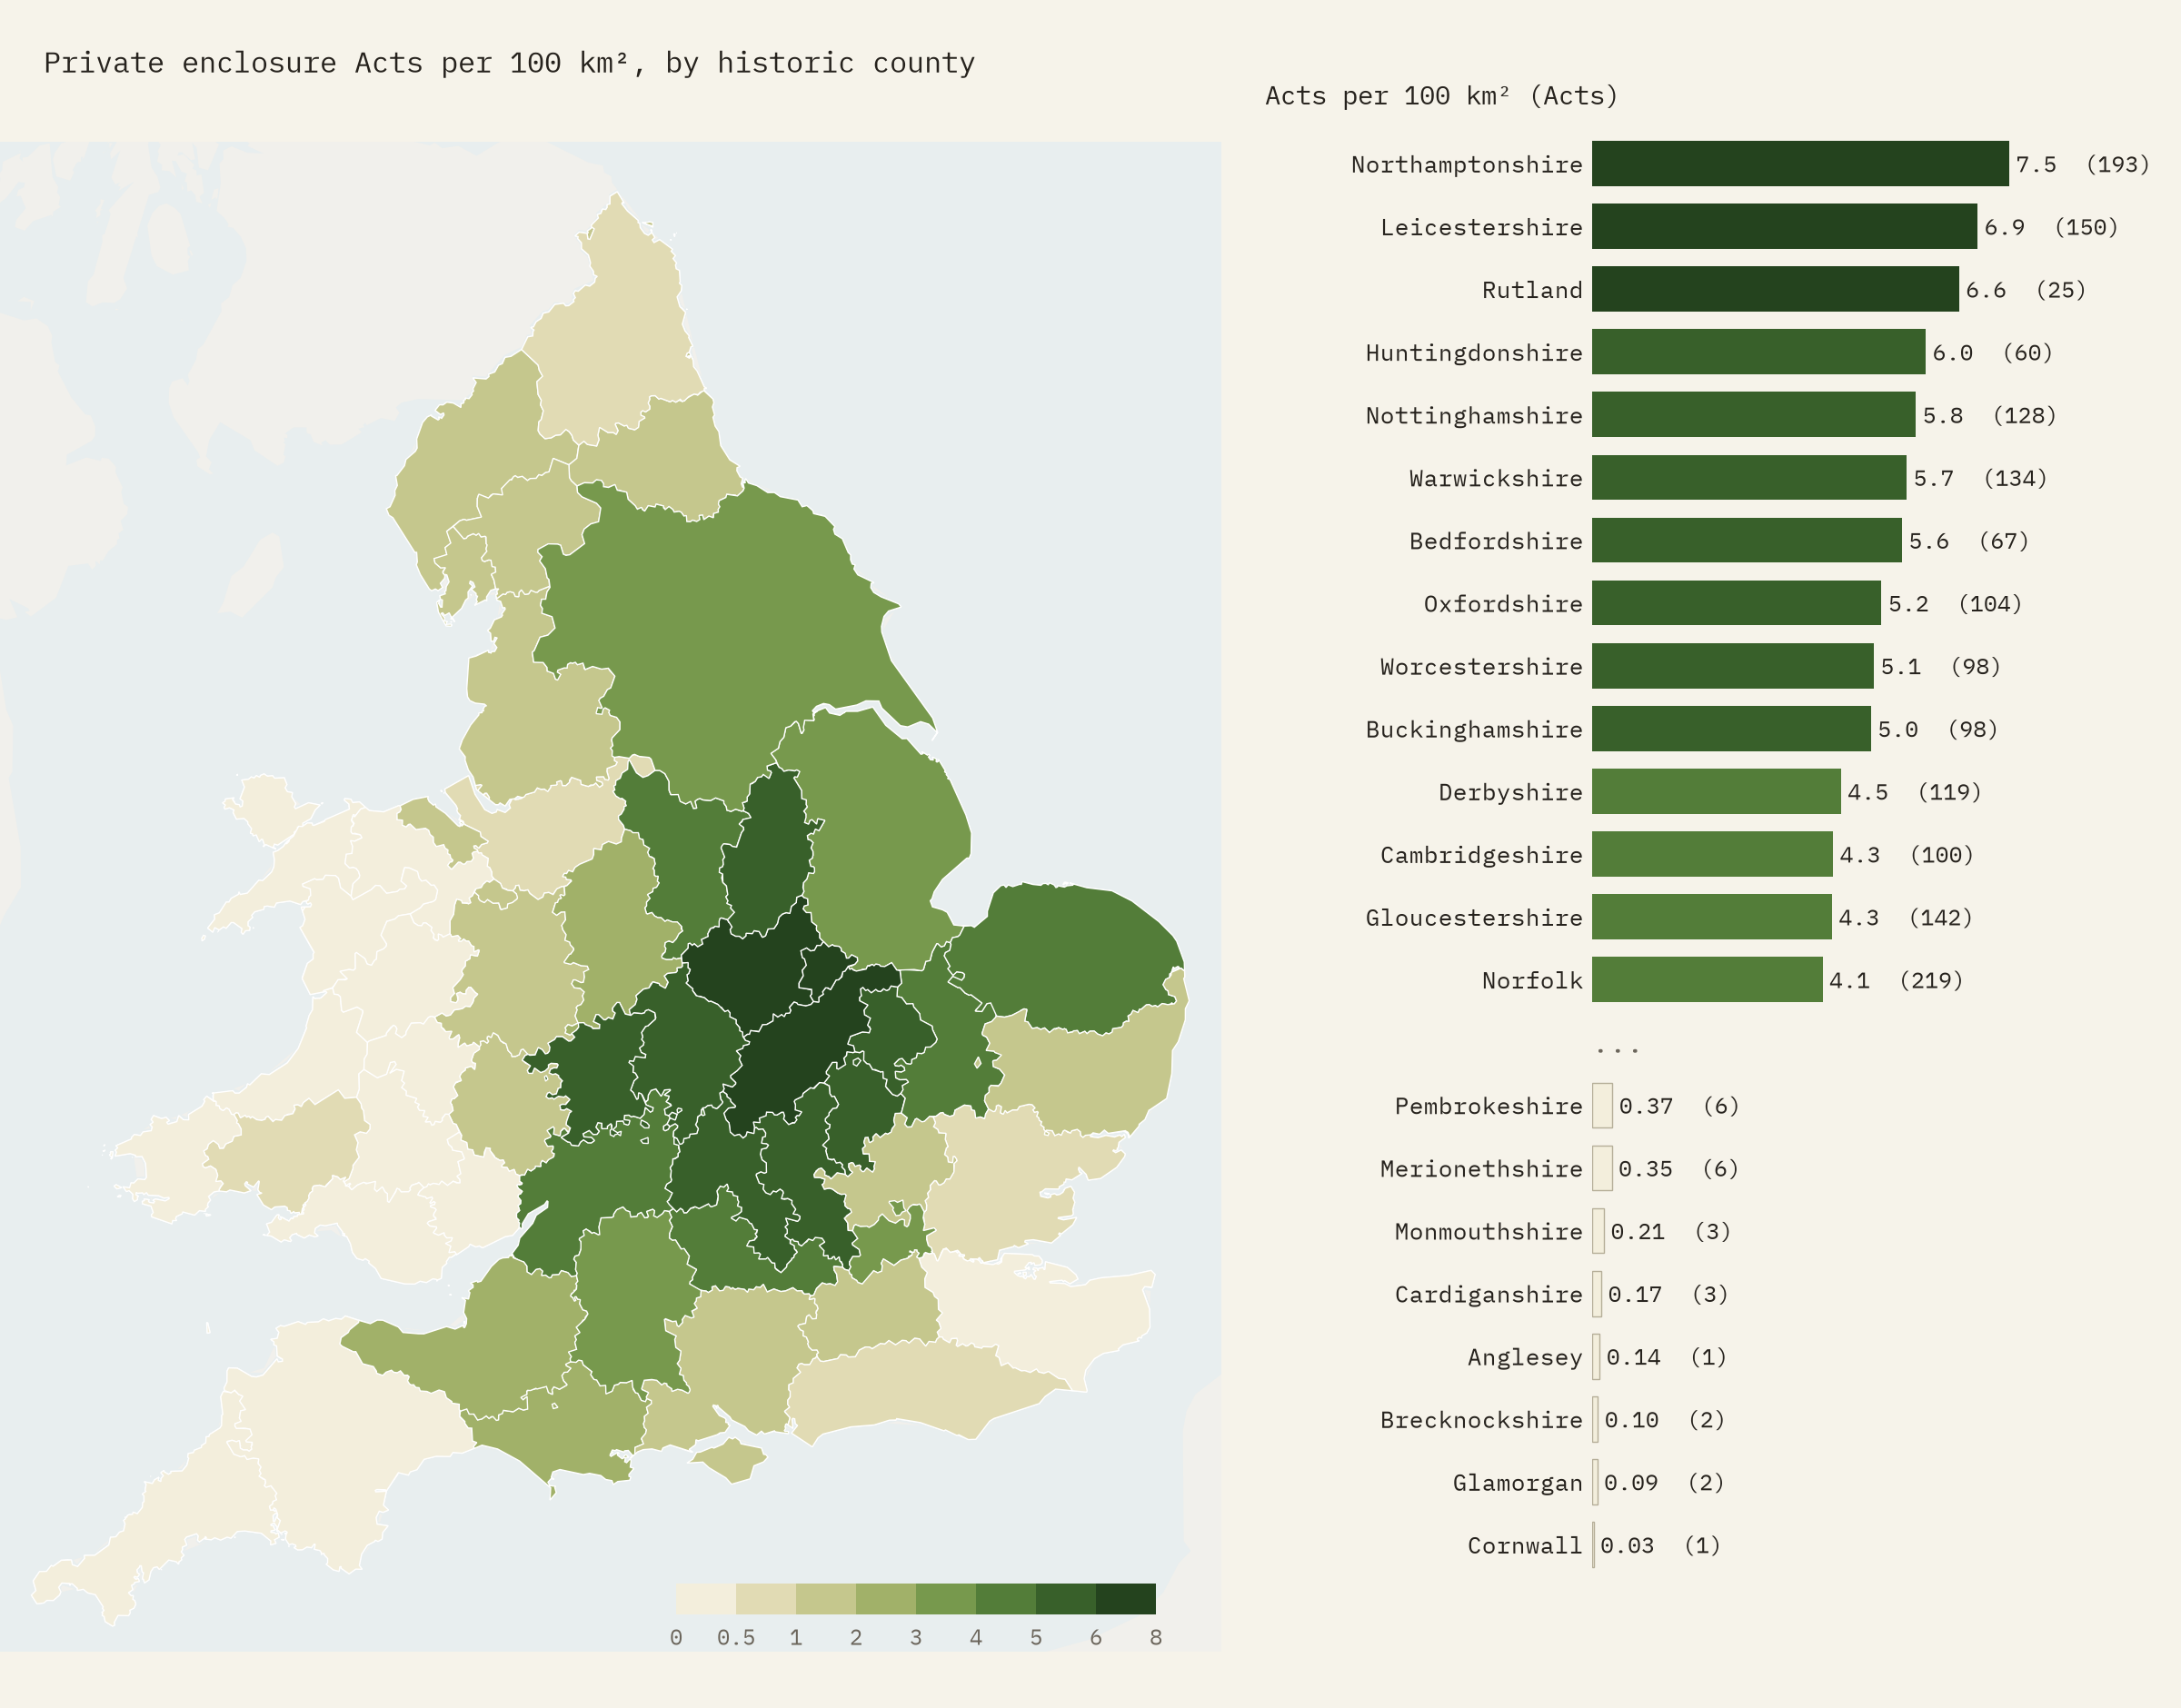
\includegraphics[width=\textwidth]{f_counties.png}
\caption{Private enclosure Acts per 100 km$^2$ by historic county (rebuilt boundaries), with the highest and lowest counties.}\label{fig:counties}\end{figure}

{\footnotesize\setlength{\tabcolsep}{4pt}\begin{longtable}{lrrrrrrrr}\caption{Enclosure Acts by historic county, ordered by private Acts per 100 km$^2$. Area from the rebuilt boundaries; first, middle and last year of all Acts; share of all Acts in the war years.}\label{tab:counties}\\\toprule County & Private & Local & km$^2$ & Per 100 km$^2$ & First & Middle & Last & War \%\\\midrule\endfirsthead\toprule County & Private & Local & km$^2$ & Per 100 km$^2$ & First & Middle & Last & War \%\\\midrule\endhead
Northamptonshire & 193 & 2 & 2,574 & 7.50 & 1727 & 1778 & 1841 & 24\\
Leicestershire & 150 & 2 & 2,164 & 6.93 & 1729 & 1772 & 1842 & 16\\
Rutland & 25 & 0 & 379 & 6.60 & 1692 & 1773 & 1820 & 44\\
Huntingdonshire & 60 & 5 & 1,000 & 6.00 & 1727 & 1800 & 1844 & 57\\
Nottinghamshire & 128 & 2 & 2,199 & 5.82 & 1758 & 1792 & 1845 & 40\\
Warwickshire & 134 & 3 & 2,370 & 5.65 & 1720 & 1775 & 1841 & 25\\
Bedfordshire & 67 & 9 & 1,203 & 5.57 & 1741 & 1800 & 1843 & 68\\
Oxfordshire & 104 & 10 & 1,999 & 5.20 & 1729 & 1793 & 1843 & 40\\
Worcestershire & 98 & 2 & 1,935 & 5.06 & 1664 & 1796 & 1833 & 40\\
Buckinghamshire & 98 & 8 & 1,955 & 5.01 & 1737 & 1796 & 1844 & 45\\
Derbyshire & 119 & 6 & 2,661 & 4.47 & 1726 & 1789 & 1841 & 26\\
Cambridgeshire & 100 & 4 & 2,308 & 4.33 & 1769 & 1811 & 1845 & 60\\
Gloucestershire & 142 & 4 & 3,292 & 4.31 & 1713 & 1795 & 1842 & 42\\
Norfolk & 219 & 42 & 5,286 & 4.14 & 1720 & 1807 & 1847 & 68\\
Berkshire & 75 & 11 & 1,848 & 4.06 & 1723 & 1802 & 1859 & 59\\
Middlesex & 28 & 3 & 735 & 3.81 & 1766 & 1811 & 1825 & 61\\
Lincolnshire & 265 & 20 & 7,014 & 3.78 & 1733 & 1786 & 1873 & 36\\
Yorkshire & 544 & 31 & 15,648 & 3.48 & 1725 & 1793 & 1844 & 39\\
Wiltshire & 115 & 9 & 3,519 & 3.27 & 1725 & 1802 & 1834 & 52\\
Somerset & 124 & 10 & 4,211 & 2.94 & 1719 & 1798 & 1842 & 62\\
Staffordshire & 76 & 6 & 3,013 & 2.52 & 1719 & 1798 & 1841 & 45\\
Dorset & 63 & 1 & 2,610 & 2.41 & 1732 & 1808 & 1837 & 61\\
Hampshire & 82 & 5 & 4,276 & 1.92 & 1709 & 1804 & 1843 & 49\\
Suffolk & 70 & 7 & 3,852 & 1.82 & 1728 & 1809 & 1839 & 75\\
Surrey & 35 & 5 & 1,954 & 1.79 & 1779 & 1806 & 1843 & 75\\
Hertfordshire & 29 & 5 & 1,652 & 1.76 & 1728 & 1801 & 1830 & 68\\
Cumberland & 67 & 10 & 3,880 & 1.73 & 1760 & 1811 & 1842 & 52\\
Herefordshire & 37 & 5 & 2,158 & 1.71 & 1772 & 1809 & 1833 & 79\\
Westmorland & 34 & 8 & 2,056 & 1.65 & 1767 & 1811 & 1838 & 45\\
Shropshire & 45 & 6 & 3,422 & 1.31 & 1764 & 1806 & 1845 & 47\\
Durham & 36 & 6 & 2,751 & 1.31 & 1756 & 1782 & 1834 & 38\\
Flintshire & 7 & 7 & 669 & 1.05 & 1775 & 1803 & 1826 & 71\\
Lancashire & 51 & 7 & 4,954 & 1.03 & 1724 & 1796 & 1830 & 47\\
Sussex & 35 & 3 & 3,813 & 0.92 & 1767 & 1809 & 1841 & 55\\
Cheshire & 23 & 10 & 2,736 & 0.84 & 1765 & 1807 & 1835 & 55\\
Essex & 32 & 3 & 4,022 & 0.80 & 1768 & 1812 & 1843 & 60\\
Northumberland & 32 & 12 & 5,224 & 0.61 & 1728 & 1792 & 1844 & 39\\
Carmarthenshire & 12 & 0 & 2,370 & 0.51 & 1807 & 1812 & 1845 & 75\\
Caernarfonshire & 7 & 2 & 1,421 & 0.49 & 1806 & 1808 & 1812 & 100\\
Montgomeryshire & 9 & 1 & 2,143 & 0.42 & 1760 & 1796 & 1832 & 40\\
Denbighshire & 7 & 4 & 1,791 & 0.39 & 1802 & 1813 & 1843 & 64\\
Radnorshire & 5 & 4 & 1,285 & 0.39 & 1810 & 1828 & 1846 & 44\\
Devon & 26 & 2 & 6,773 & 0.38 & 1799 & 1813 & 1842 & 64\\
Kent & 15 & 3 & 4,025 & 0.37 & 1562 & 1810 & 1840 & 50\\
Pembrokeshire & 6 & 1 & 1,638 & 0.37 & 1786 & 1809 & 1832 & 57\\
Merionethshire & 6 & 0 & 1,696 & 0.35 & 1805 & 1807 & 1810 & 100\\
Monmouthshire & 3 & 0 & 1,403 & 0.21 & 1776 & 1808 & 1813 & 67\\
Cardiganshire & 3 & 0 & 1,803 & 0.17 & 1812 & 1813 & 1815 & 100\\
Anglesey & 1 & 2 & 725 & 0.14 & 1812 & 1814 & 1815 & 100\\
Brecknockshire & 2 & 1 & 1,897 & 0.10 & 1807 & 1814 & 1814 & 100\\
Glamorgan & 2 & 0 & 2,123 & 0.09 & 1762 & 1797 & 1833 & 0\\
Cornwall & 1 & 1 & 3,608 & 0.03 & 1809 & 1813 & 1818 & 50\\
\bottomrule\end{longtable}}

\subsection{The geography of the second wave}
Figure~\ref{fig:waves} compares 1750 to 1779 with the war years. The Midland belt's share fell from 52.6\% to 31.1\%, the north's from 25.7\% to 18.9\%. Norfolk and Suffolk rose from 2.4\% to 12.8\%, the south-west and Welsh border from 11.9\% to 22.2\%, the home counties and Kent from 1.5\% to 6.7\%, and Wales from 0.4\% to 3.5\%. Located Acts west of 2$^\circ$W rose from 13.2\% to 26.6\%. Acts naming more than one place became more common (16\% to 24\%). The historiography describes the war-years enclosures as reaching further into commons, heaths and wastes \citep{turner1980}; the titles cannot test that directly, since only 5.2\% of all enclosure titles name a common, moor, heath, fen, forest or similar land, and that share did not rise in the war years (5.9\% against 3.8\%).

\begin{figure}[tbp]\centering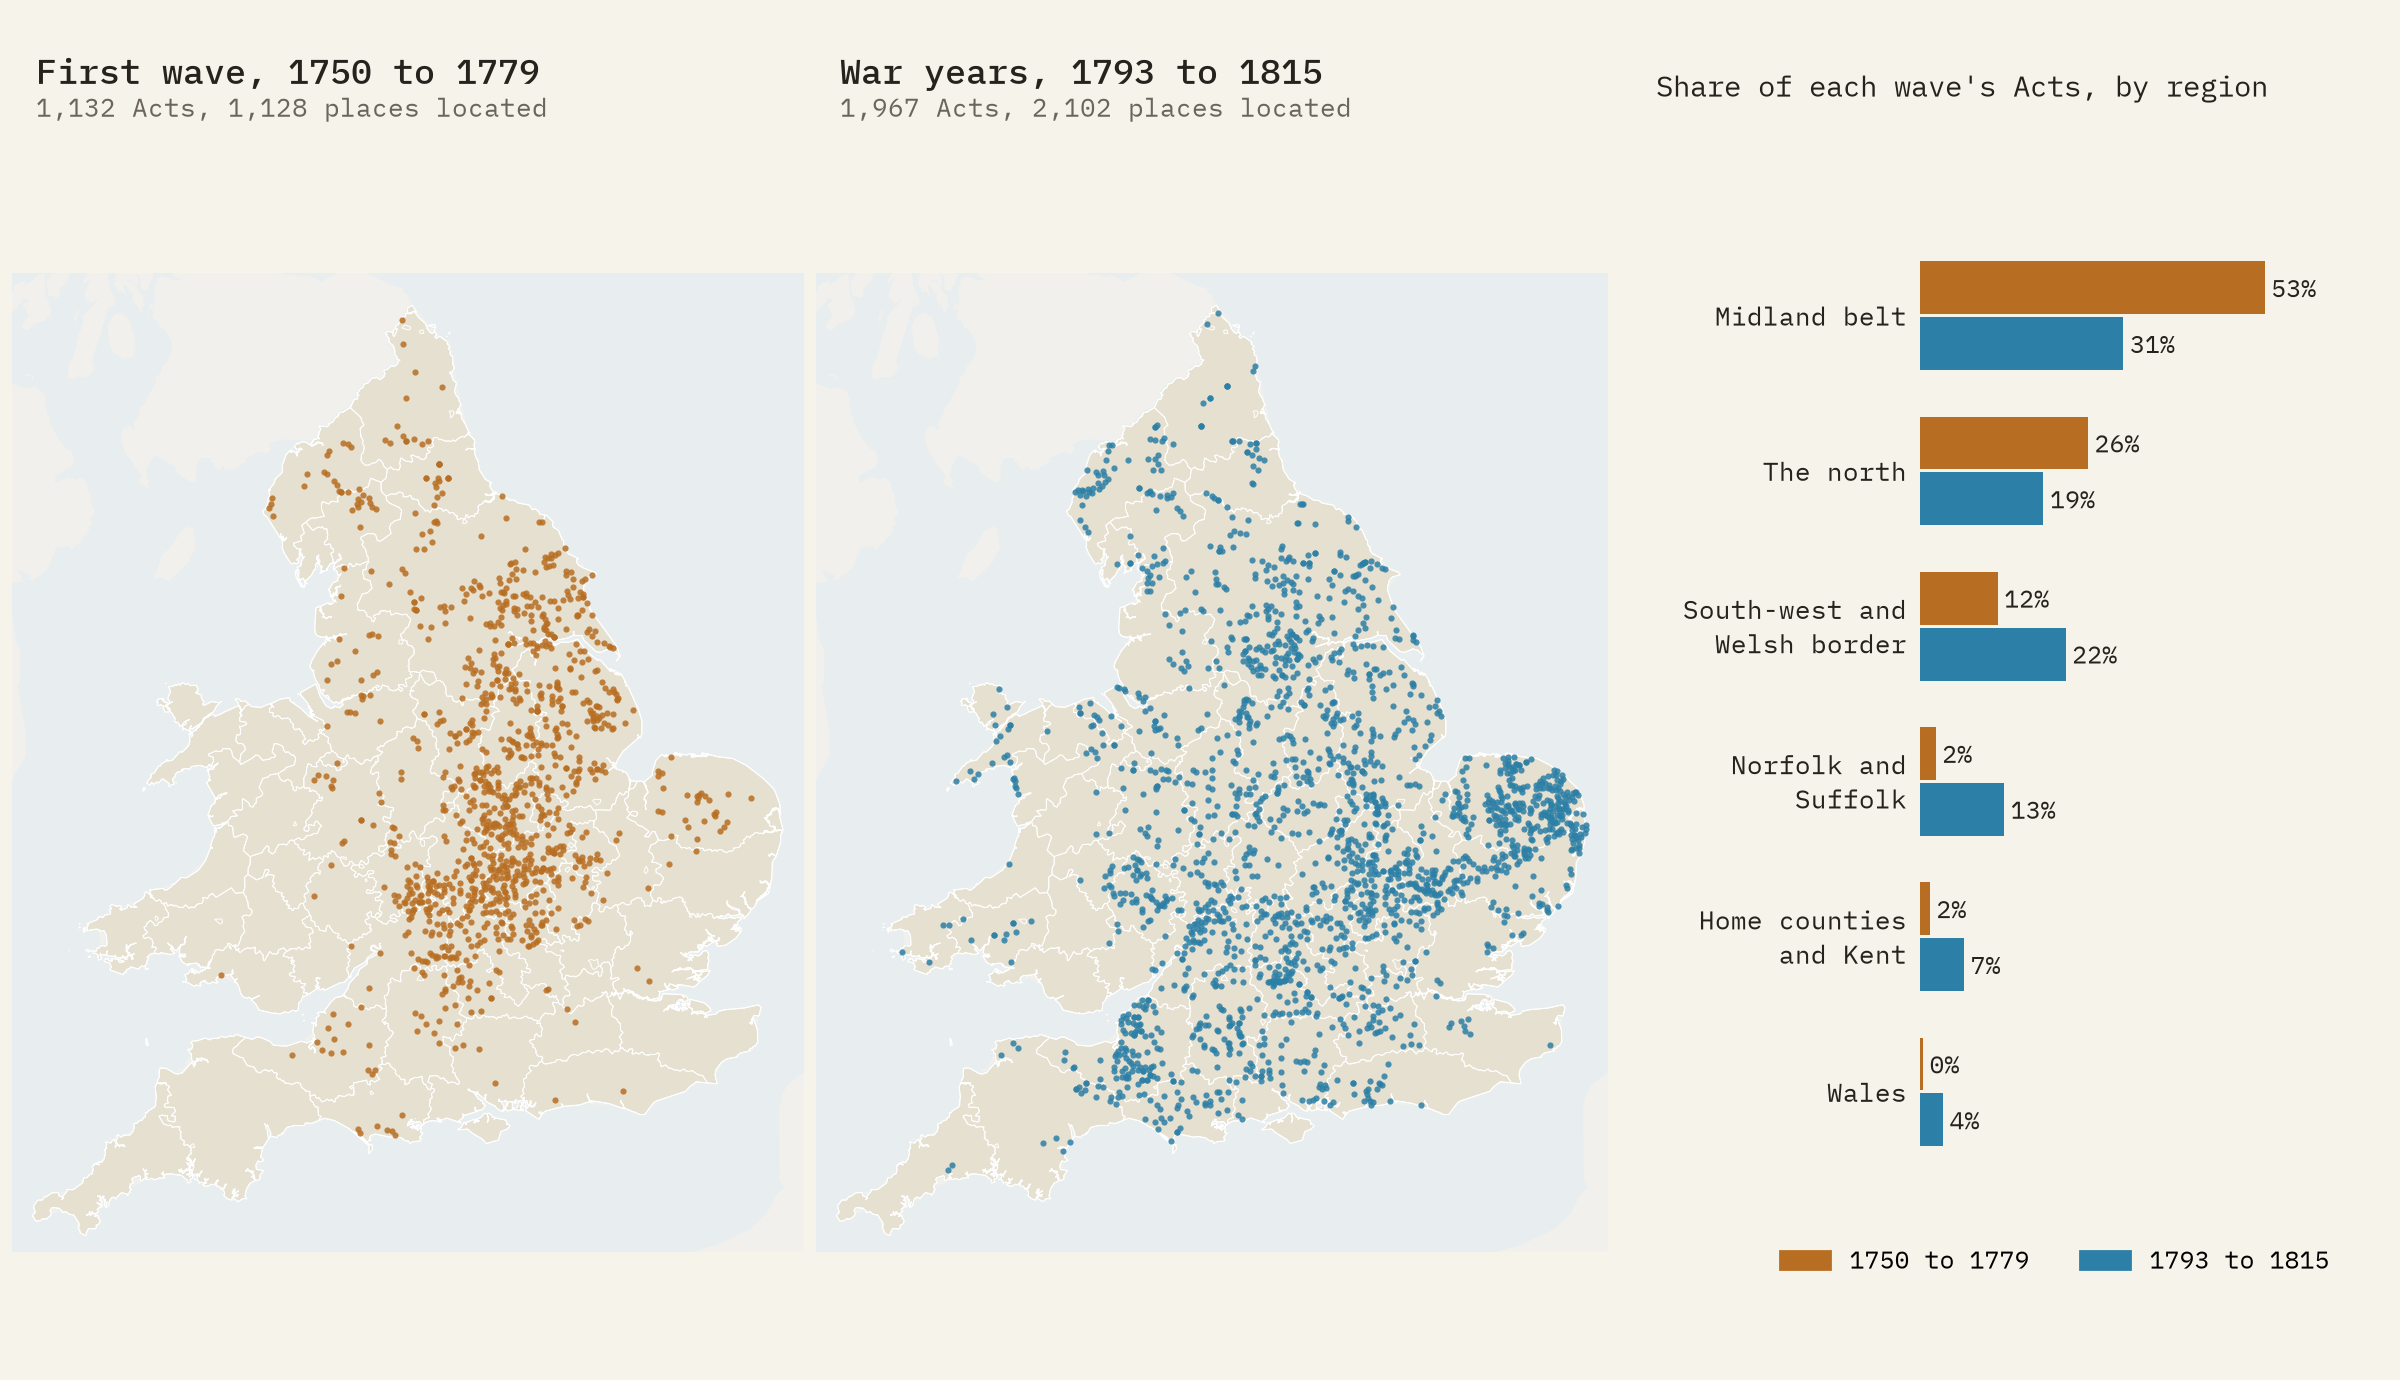
\includegraphics[width=\textwidth]{f_waves.png}
\caption{Located places in Acts of 1750 to 1779 and of 1793 to 1815, with each period's share of Acts by region.}\label{fig:waves}\end{figure}

\subsection{The moving centre}
The decade centroids (Figure~\ref{fig:centroid}) stay within the East Midlands throughout. In the 1760s the centre lay near Carlton on the edge of Nottingham, drawn north by Yorkshire and Lincolnshire; by the 1810s it lay 46 km away, near Earl Shilton west of Leicester (about 45 km south and 12 km west); in the 1830s and 1840s it was near Rugby.

\begin{figure}[tbp]\centering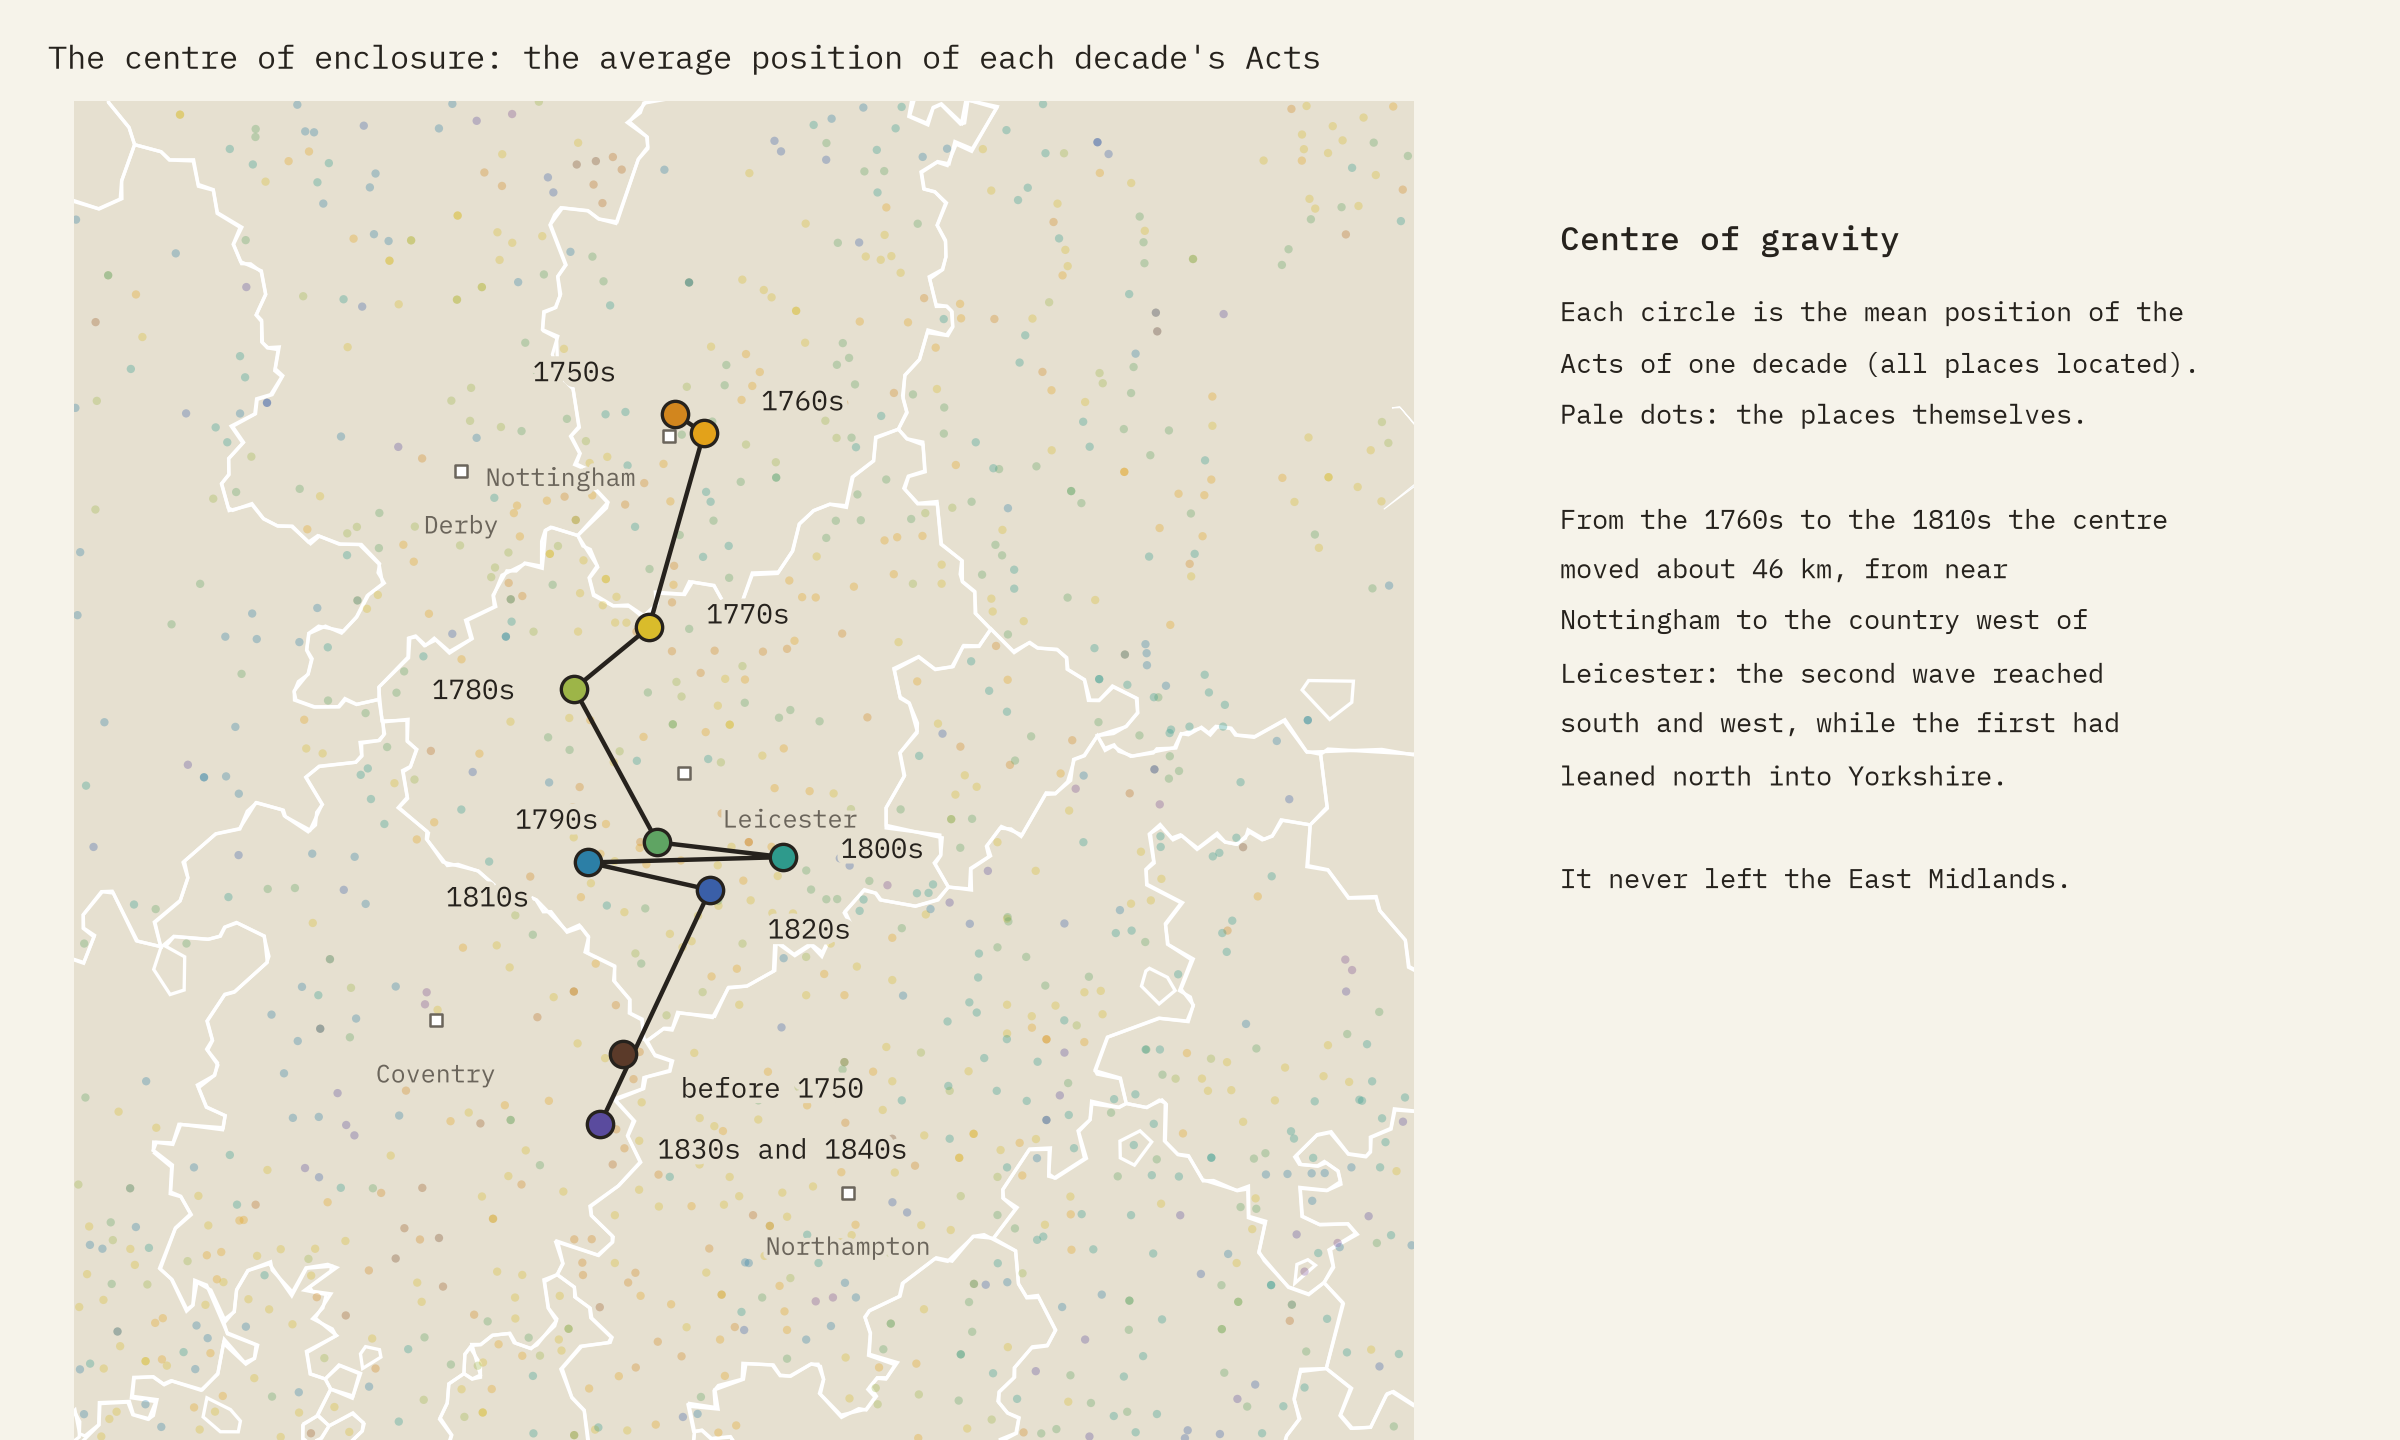
\includegraphics[width=\textwidth]{f_centroid.png}
\caption{Mean position of the located Acts of each decade.}\label{fig:centroid}\end{figure}

\subsection{Cases}
The earliest title in the private table that mentions enclosure is the 1562 Act for Plumstead Marsh in Kent, a marsh drainage and embanking scheme; there are 5 Plumstead Marsh Acts in all. The first title of the familiar form after it is Ropley Commons (Hampshire) in 1709. The last private enclosure Act is for Terrington in Norfolk in 1847, and the last local enclosure Act is for Gedney in Lincolnshire in 1873; later enclosures went through the Inclosure Commissioners. 871 Acts (21\%) name more than one place; the longest list is the 1811 Act naming 10 places around Shenstone in Staffordshire. 258 gazetteer places are named in enclosure Acts of two or more different years and 25 in three or more (Figure~\ref{fig:twice}); Elsdon, Simonburn and Rothbury in Northumberland, Chatteris in Cambridgeshire and Lanchester in Durham appear in four. The longest interval is at Eccleshall in Staffordshire, between Acts of 1719 and 1841.

\begin{figure}[tbp]\centering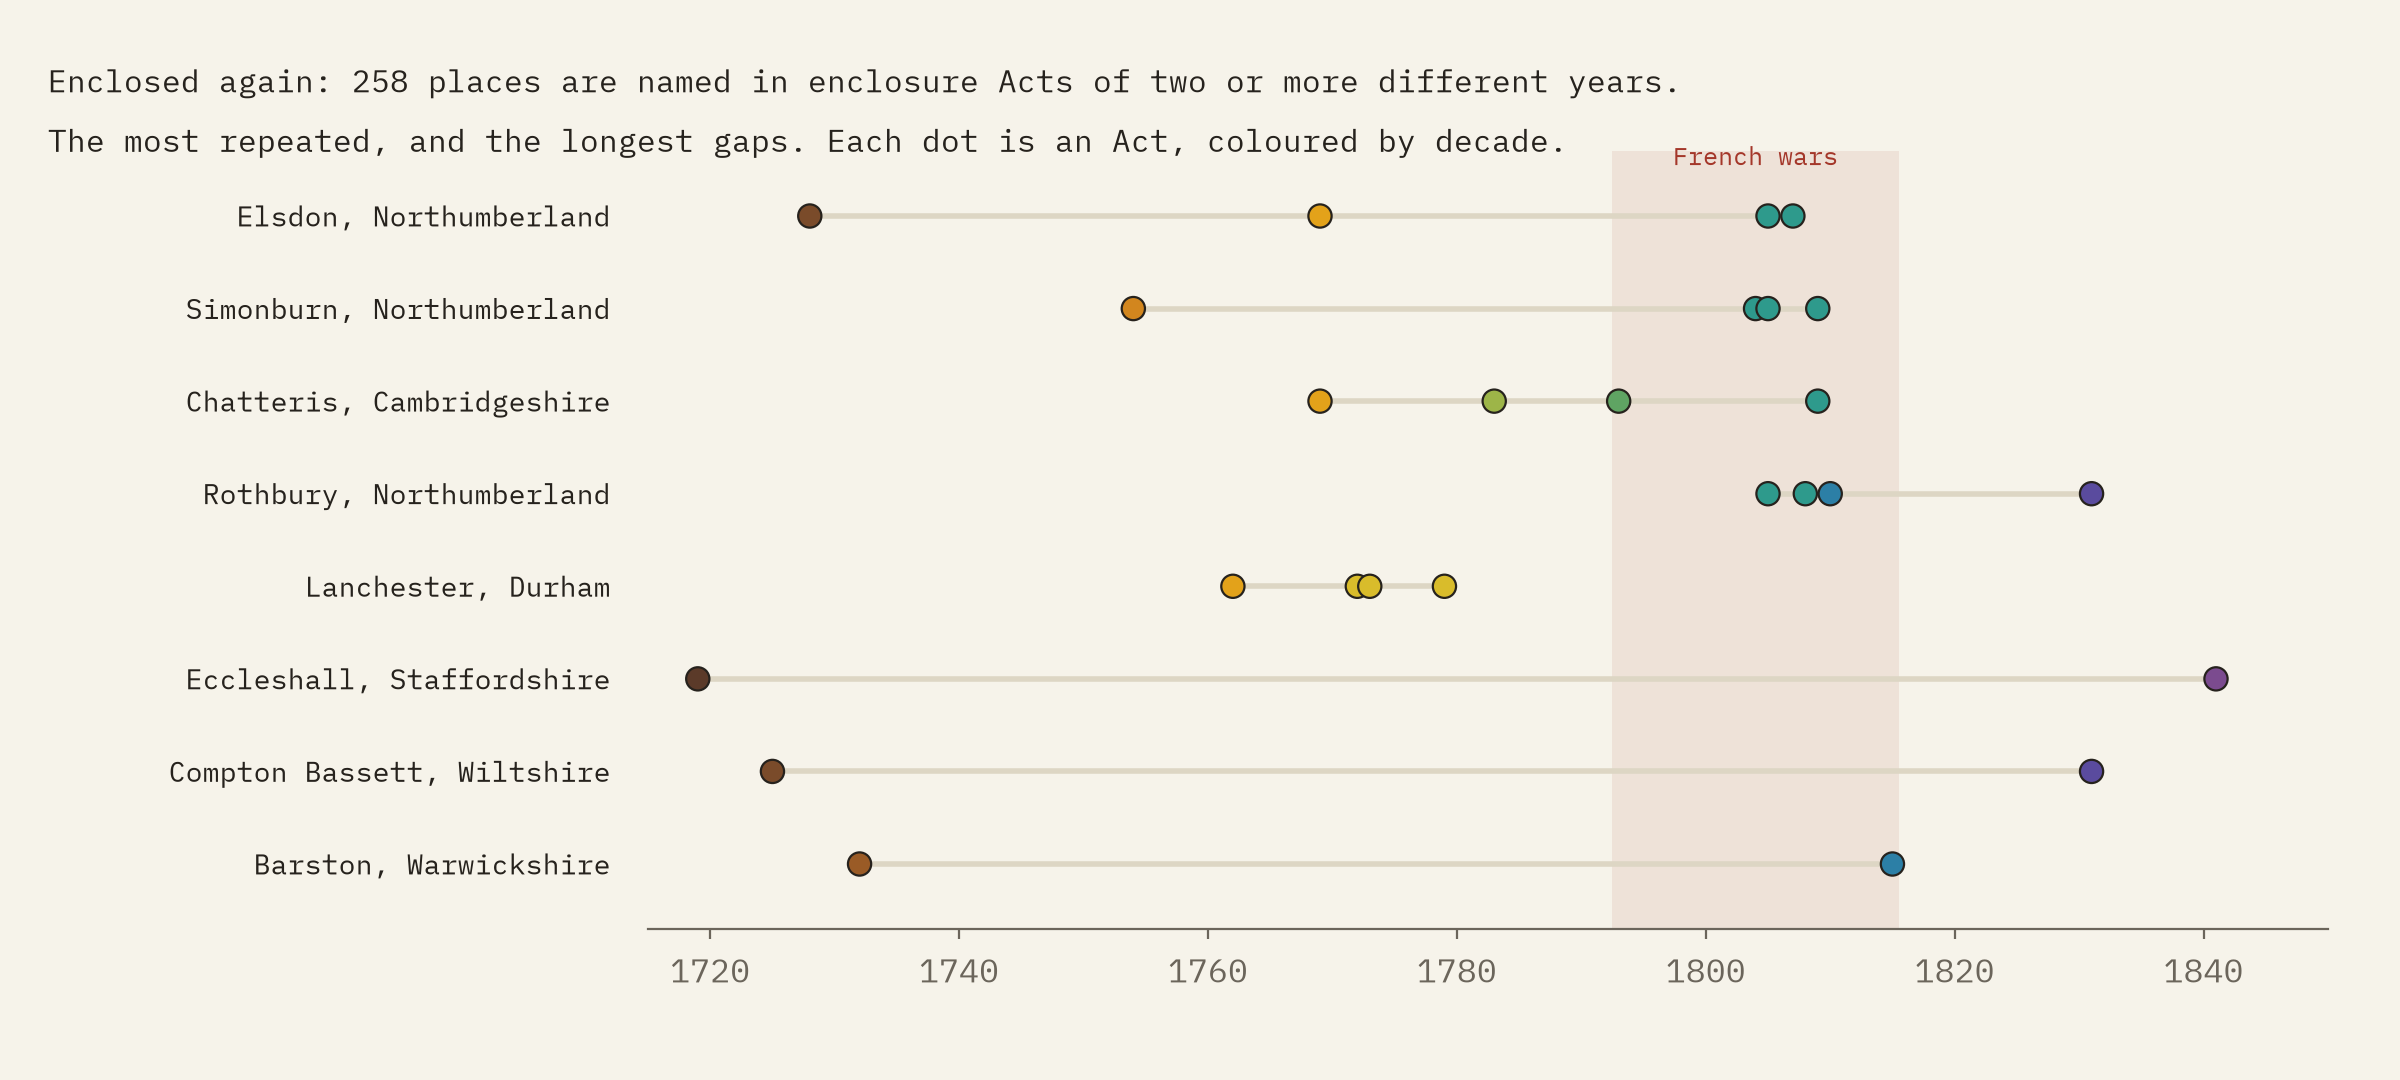
\includegraphics[width=\textwidth]{f_twice.png}
\caption{Places named in several enclosure Acts: the most repeated and the longest gaps.}\label{fig:twice}\end{figure}

\section{Discussion}
The pattern is the familiar one from the county studies, recovered here from a single open source: a Midland belt of open-field parishes enclosed mainly in the first wave, and a second wave in the French wars that reached further south, east and west, into Norfolk and Suffolk, the south-west, the home counties and Wales. The interpretation of that pattern is not settled by counting Acts. Enclosure allowed consolidation, drainage and new rotations, and studies have found that output and rents rose where it occurred \citep{chambers1966,turner1980}; Allen argued that the productivity gains were modest and that most of the extra income went to landowners as rent \citep{allen1992}. Enclosure also extinguished common rights of grazing, fuel and gleaning that mattered to cottagers and labourers, many of whom received little or nothing in the allotment \citep{hammond1911,neeson1993}. Both effects are consistent with the map: the same Acts that fenced fields for higher output fenced commons that the poor had used.

\section{Limitations}
First, this is a count of Acts as two chronological tables list them, not a count of enclosures. The total commonly quoted for England, more than 5,000 Acts, draws on Tate's and Turner's work and also includes public local Acts and enclosures completed after 1845 by the Inclosure Commissioners, confirmed by general Acts that the tables do not itemise; enclosure by agreement without an Act does not appear. Second, two pages of the local table are missing, so local Acts for 1802 to 1803 and for 1841 are not counted. Third, titles are classified by rule; a few borderline titles may be misclassed, and 68 allotment titles are excluded. Fourth, 79\% of named places were located; local Acts (65\%) and Welsh places (57\%) match less well, so their weight on the maps is understated. Fifth, county areas come from rebuilt boundaries. Sixth, an Act counts once whatever its acreage, so a small Act for one common weighs as much as one that enclosed a whole parish.

\section{Conclusion}
The Chronological Tables provide a free, reproducible way to map parliamentary enclosure in England and Wales. They show two waves, the second larger and wider than the first, a Midland heartland, and a late and partial reach into the south-west and Wales. Combining the private and local tables is essential: on its own the private table hides half of the war-years boom.

\section*{Data and code availability}
The interactive map is at \url{https://maps.tristanhotham.com/enclosure/}. Data and code are at \url{https://github.com/Tristan-Hotham/enclosure} and archived with this paper at https://doi.org/10.5281/zenodo.23873003. Derived data and text are released under CC BY 4.0 and code under the MIT licence. The chronological tables are Crown copyright, used under the Open Government Licence v3.0; Wikidata is CC0.

\section*{AI statement}
I wrote the text, with drafting and editing assistance from Claude (Anthropic), which also helped prepare the analysis code. I reviewed and checked all text and results.

\begin{thebibliography}{9}
\bibitem[Allen(1992)]{allen1992} Allen, R. C. (1992) \textit{Enclosure and the Yeoman: The Agricultural Development of the South Midlands, 1450 to 1850}. Oxford: Clarendon Press.
\bibitem[Chambers and Mingay(1966)]{chambers1966} Chambers, J. D. and Mingay, G. E. (1966) \textit{The Agricultural Revolution 1750 to 1880}. London: Batsford.
\bibitem[Hammond and Hammond(1911)]{hammond1911} Hammond, J. L. and Hammond, B. (1911) \textit{The Village Labourer 1760 to 1832}. London: Longmans, Green.
\bibitem[legislation.gov.uk(2026a)]{legpriv} legislation.gov.uk (2026) Chronological Table of Private and Personal Acts. Crown copyright, Open Government Licence v3.0. \url{https://www.legislation.gov.uk/changes/chron-tables/private}
\bibitem[legislation.gov.uk(2026b)]{legloc} legislation.gov.uk (2026) Chronological Table of Local Acts. Crown copyright, Open Government Licence v3.0. \url{https://www.legislation.gov.uk/changes/chron-tables/local}
\bibitem[Neeson(1993)]{neeson1993} Neeson, J. M. (1993) \textit{Commoners: Common Right, Enclosure and Social Change in England, 1700 to 1820}. Cambridge: Cambridge University Press.
\bibitem[Tate(1978)]{tate1978} Tate, W. E. (1978) \textit{A Domesday of English Enclosure Acts and Awards}, ed. M. E. Turner. Reading: University of Reading.
\bibitem[Turner(1980)]{turner1980} Turner, M. (1980) \textit{English Parliamentary Enclosure: Its Historical Geography and Economic History}. Folkestone: Dawson.
\bibitem[Wikidata(2026)]{wikidata} Wikidata contributors (2026) Places in the United Kingdom with coordinates and historic county (P7959). CC0. \url{https://www.wikidata.org/}
\end{thebibliography}
\end{document}
